\section{Tsai Camera Model}

A camera model is a projection model which describes a mathematical relationship between points in 3D space and its projection onto an image plane. There are many variation of a 

The Tsai camera model builds upon the pinhole camera model, which is one of the simplest and most commonly used camera models.

\subsection{Pinhole Camera}

A pinhole camera is a simple camera without a lens. Instead, it has a small aperture, and light rays pass through the aperture and projects an inverted image 

\begin{figure}[h!]
    \centering
    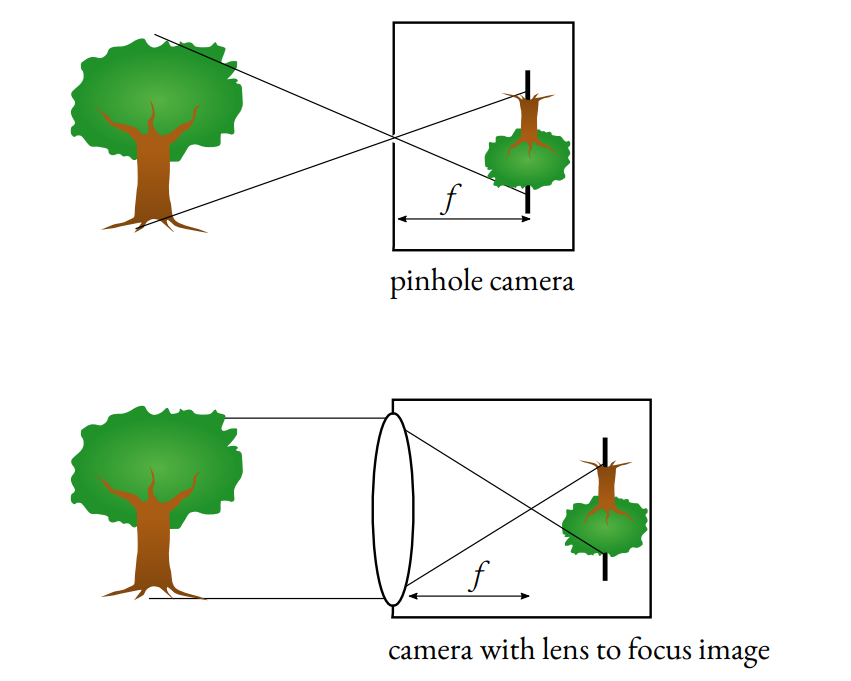
\includegraphics[width=0.7\textwidth]{images/pinhole_vs_lens}
    \caption{Difference between a pinhole camera and a lens camera}
\end{figure}



There are a few assumptions which are made by the pinhole camera model:
\begin{itemize}
    \item T
\end{itemize}

The pinhole camera model does not accurately describe the true workings of a camera, as some of the  effects that the model fails to account for can be compensated the errors which results from these assumptions are sufficiently small to be neglected if a high quality camera is used. Additionally,

\subsection{Nomenclature}

\begin{figure}[h!]
    \centering
    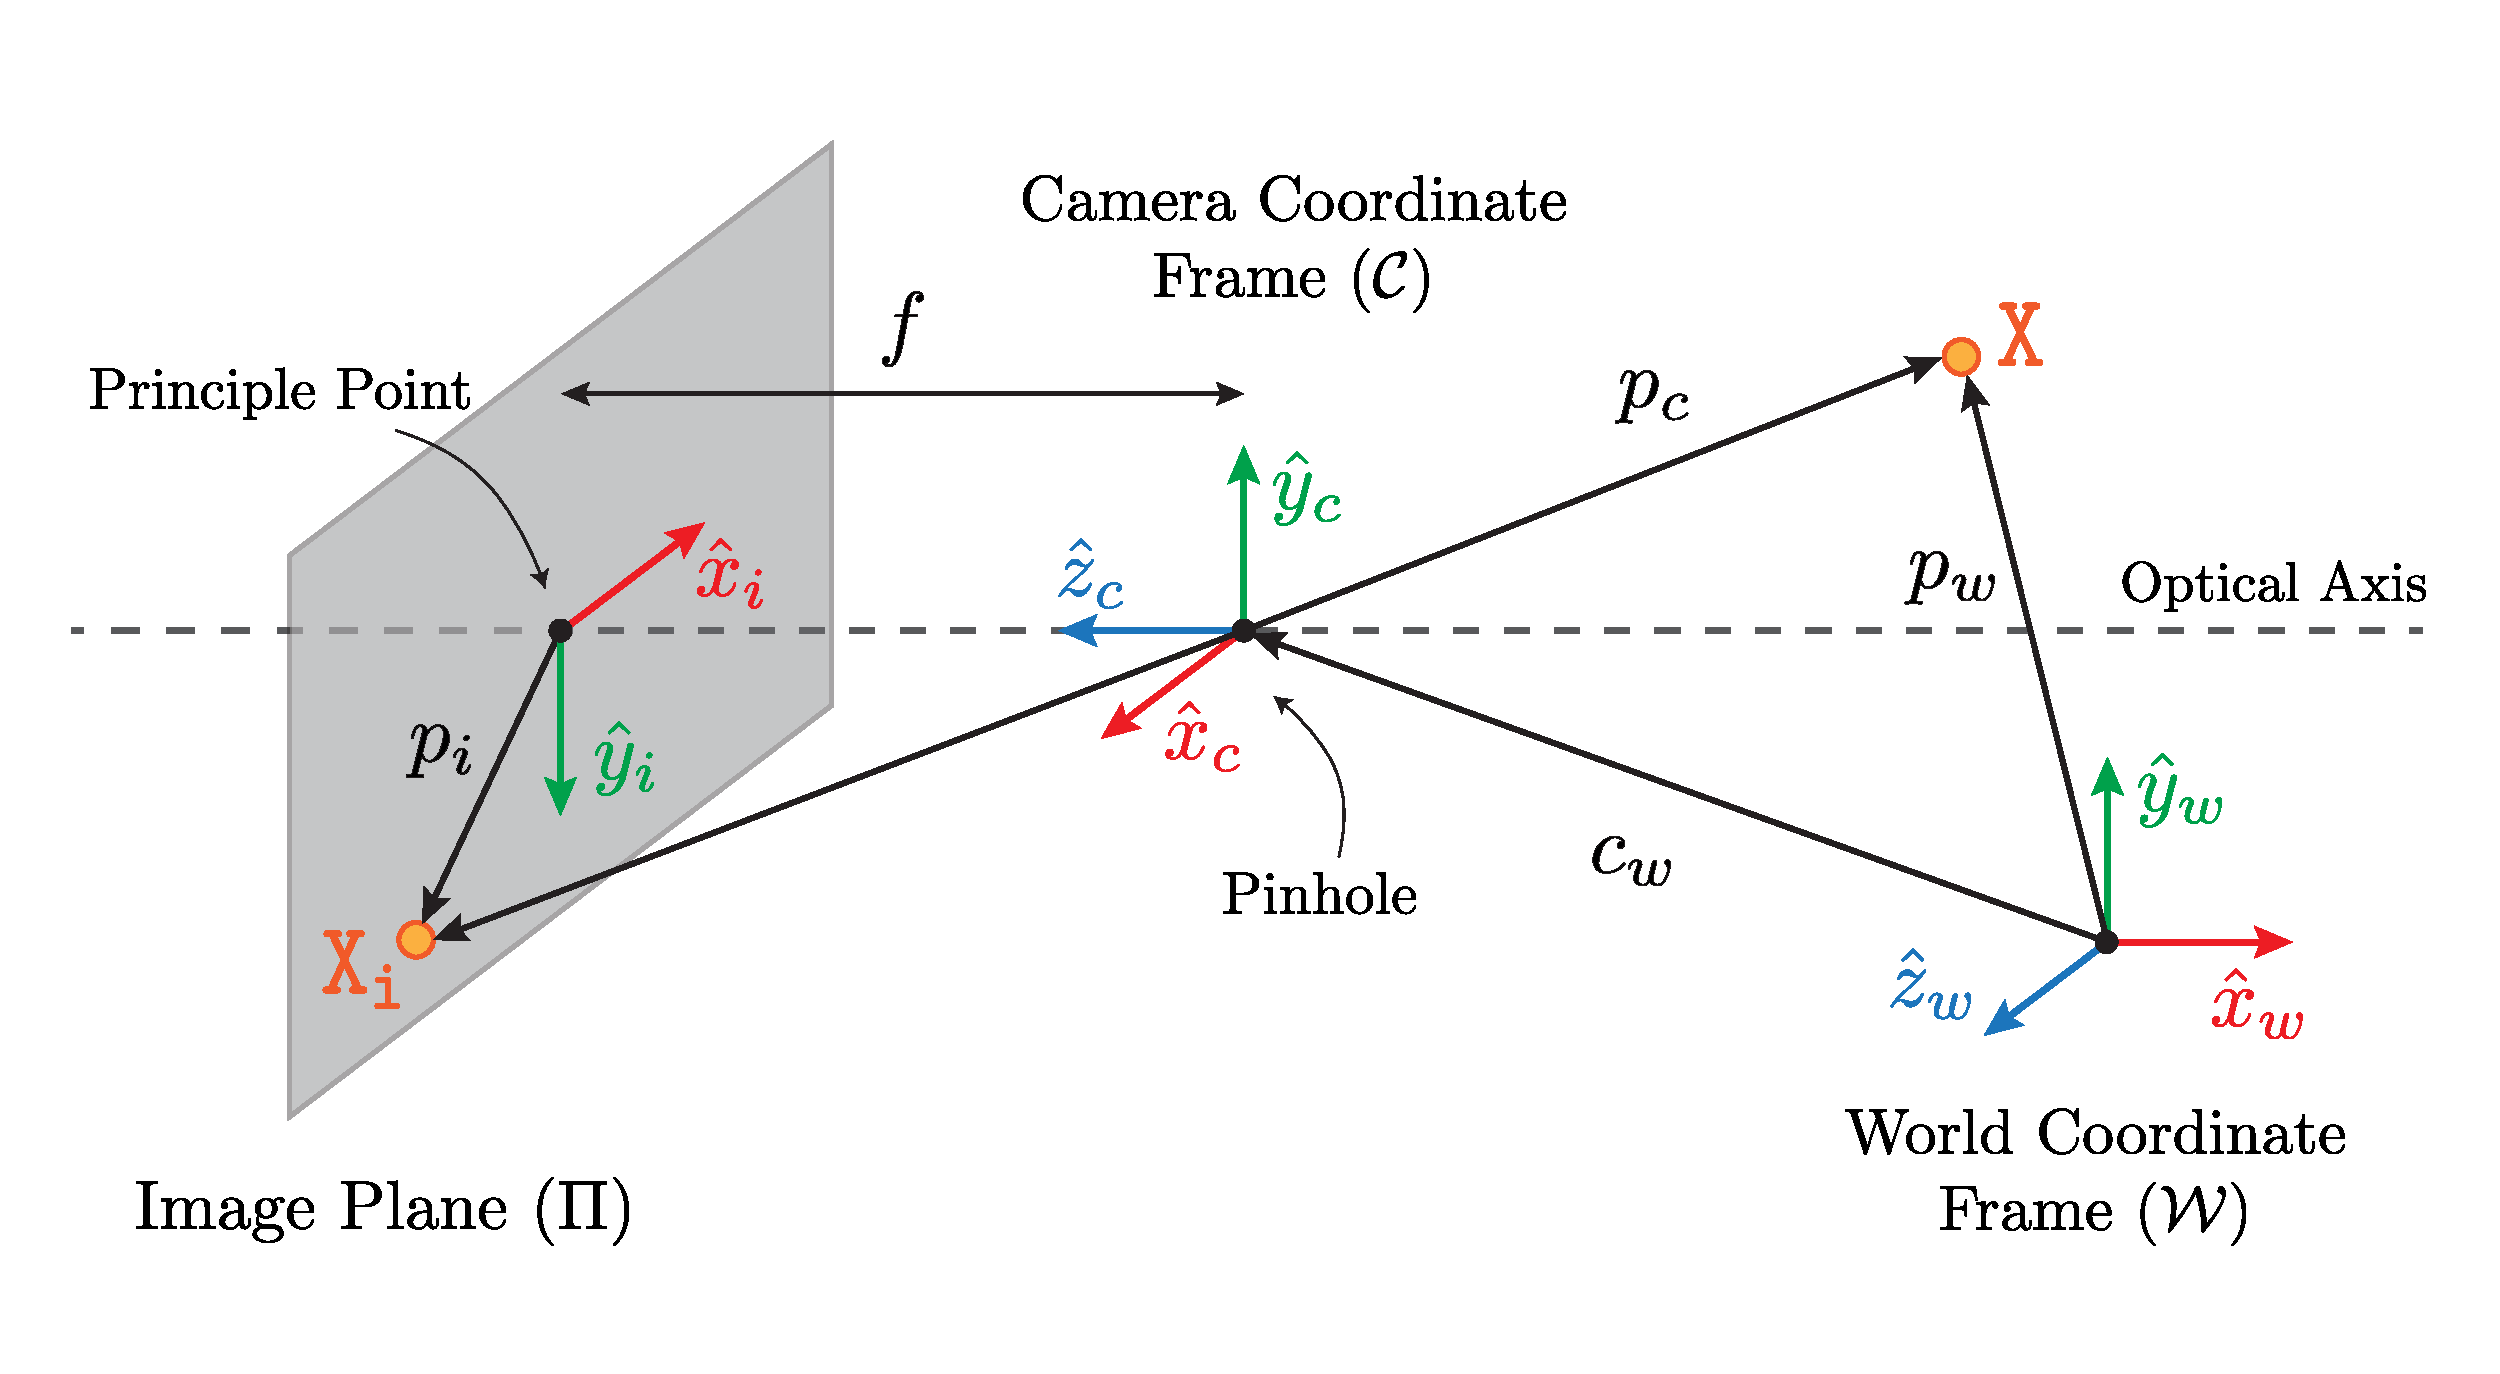
\includegraphics[width=0.9\textwidth]{figures/imaging_model}
    \caption{Pinhole Camera Model}
\end{figure}


